\documentclass{article}

\usepackage{geometry,graphicx,amsmath,amssymb}
\usepackage{tikz}
% TikZ (TikZ ist kein Zeichenprogramm/TikZ is not drawing program),can use to draw graph
% the TikZ based on PGF(Portable Graphics Format) command

\author{YL-TING}
\title{Learning LaTeX - Day8}
\date{\today}

\begin{document}
    \maketitle
    \newpage

    % Part1

    % the TikZ picture is inline object,but we also can put in any place that is up to myself
    % every line command in tikz block need ; in the end
    {\Large Tikz}\\[10pt]
    There is a red dot 
    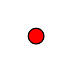
\begin{tikzpicture}
        \draw[fill=red] (0,0) circle (0.1);
    \end{tikzpicture}
    in the middle of this sentence.\\[15pt]

    {\Large Basic Lines in Tikz}\\[10pt]
    % the TikZ picture is based on 2D-coordinate system,up is +y,right is +x,default unit is cm
    \begin{tikzpicture}
        \draw (0,0) -- (3,2);
        %    start line end
    \end{tikzpicture}

    % Multiple Lines
    \begin{tikzpicture}
        \draw (0,0) -- (3,0) % 1st point to 2nd point
                    -- (3,4) % 2nd point to 3rd point
                    -- (0,4) % 3rd point to 4th point
                    -- cycle;% use cycle to close the loop,that is better than -- (0,0)
        % is same as \draw (0,0) -- (3,0) -- (3,4) -- (0,4) -- cycle;
    \end{tikzpicture}\\[15pt]
    {\Large Polar Coordinates}\\[10pt]
    % (angle : radius)
    \begin{tikzpicture}
        \draw (0:2) -- (45:2) -- (90:2)
          --(135:2) -- (180:2) -- (225:2)
          --(270:2) -- (315:2) --cycle;
    \end{tikzpicture}

    {\Large Relative Coordinates}\\[10pt]
    % use ++ to use relative coordinate,the ref point(origin) is the previous point
    % the drawing path in relative coodinate is not unique
    \begin{tikzpicture}
        \draw (0,0) -- ++(2,0) -- ++(0,2);
        % the graph is equal to 
        \draw (3,0) -- ++(2,0) -- ++(0,2); 
        % and equal to
        \draw (-3,0) -- ++(2,0) -- ++(0,2);
    \end{tikzpicture}
    \begin{tikzpicture}
        \draw (45:2) ++(30:3) -- ++(4,0);
        % its will not display the line without -- but point is linked
    \end{tikzpicture}\\[15pt]

    \newpage

    {\Large Shapes}\\[10pt]
    \begin{tikzpicture}
        \draw (-2,-1) rectangle (2,1);
        % two oppsite corner topleft-bottomright or bottomleft-topright
    \end{tikzpicture}
    \begin{tikzpicture}
        \draw (0,0) circle (2); % old notation
        %   center          radius
        \draw (0,0) circle [radius=2]; % new notation
    \end{tikzpicture}
    \begin{tikzpicture}
        \draw (0,0) circle (4 and 2); % old notation
        \draw (0,0) circle [x radius=4,y radius=2]; % new notation
    \end{tikzpicture}\\[15pt]

    {\Large Drawing Circular and Elliptical Arcs}\\[10pt]
    \begin{tikzpicture}
        \draw (0,0) arc (0:135:2); % old notation
        %   start pt      (start angle:end angle:radius)
        \draw (0,0) arc [radius=2,start angle=0,end angle=135]; % new notation
    \end{tikzpicture}
    \begin{tikzpicture}
        \draw (0,0) arc (180:45:4 and 2); % old notation
        \draw (0,0) arc [x radius=4,y radius=2,start angle=180,end angle=45]; % new notation
        % for ellipse,the sequence of parameter is not important
        % the angle is not ref to center of ellipse,is ref to the circle that stretched out into the ellipse
    \end{tikzpicture}\\[15pt]

    {\Large Nodes}\\[10pt]
    % node is a container for displaying logic objects
    % most of time this is used to contain text or equations
    % need to specify the location of node and create a container
    % whatever put in the container is what will be display at that point
    % ways to create node: using node,path,coordinate command
    % can also set node name and use as another way to indicate location
    \begin{tikzpicture}
        \draw (0,0) node {Node A};
        \draw (0,2) node {Node B};
        \draw (3,2) node {Node C};
    \end{tikzpicture}
    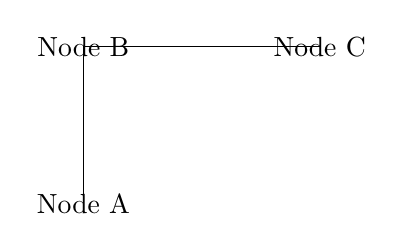
\begin{tikzpicture}
        \draw (0,0) node {Node A}
            --(0,2) node {Node B}
            --(3,2) node {Node C};
    \end{tikzpicture}
    % if don't want text overlap the line ,can use fill option
    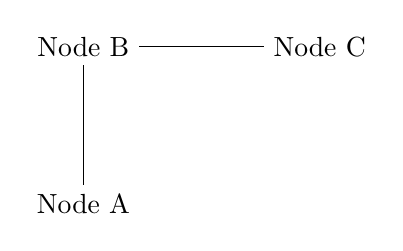
\begin{tikzpicture}
        \draw (0,0) node[fill=white] {Node A}
            --(0,2) node[fill=white] {Node B}
            --(3,2) node[fill=white] {Node C};
    \end{tikzpicture}\\

    % coordinate
    % coordinate names shown for clarity,they do not automatically display
    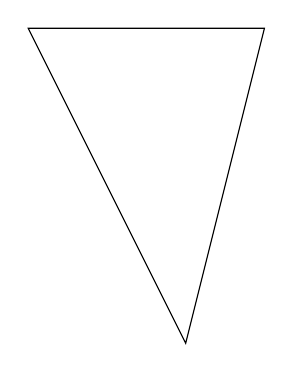
\begin{tikzpicture}
        \coordinate (A) at (2,0);
        \coordinate (B) at (0,4);
        \coordinate (C) at (3,4);
        \draw (A)--(B)--(C)--cycle;
    \end{tikzpicture}

    \newpage

    {\Large Node Positioning}\\[10pt]
    % we can change the position of nodes anchor(定位點或錨點),defaukt is center of the textjust above the coordinate
    \includegraphics[width=1.2\linewidth]{node_position.png}

    \newpage
    
    % Part2

    % Predefined Colors in TikZ
    % use \draw[color_name] ... ;
    % primary and secondary
    %   red,yellow,green,cyan,blue,violet
    % other color
    %   megenta,brown,lime,olive,orange,pink,purple,teal
    % grayscale
    %   white,lightgray,gray,darkgray,black

    % Custom Colors in TikZ
    % RGB colors
    %   use \draw[fill={rgb,255:red,21;green,66;,blue,128}]
    % if use some color frequently,can use
    % \definecolor{mycolor_name}{RGB}{21,66,128}
    % Mixing colors
    %   color1!persenttage_of_color1!color2
    %   example : blue!75!white is mean 75% blue mix 25% white

    {\Large Filling Shapes}\\[10pt]
    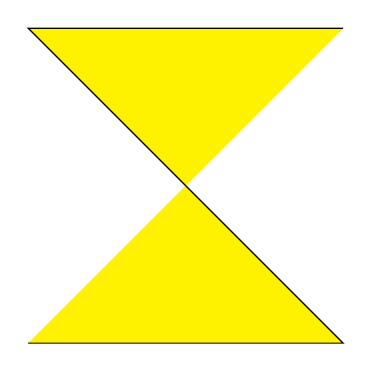
\begin{tikzpicture}
        \draw[fill=yellow] (0,0) -- (4,0) -- (0,4) -- (4,4);
        % if figure is not closed,there is no black line connecting the last pt to the first pt
    \end{tikzpicture}
    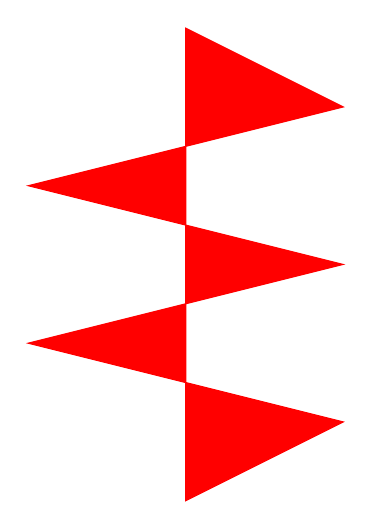
\begin{tikzpicture}
        % line color,fill color
        \draw[red,fill=red] (0,0) --(0,6) --(2,5) --(-2,4) --(2,3)
                         --(-2,2) --(2,1) --cycle;
    \end{tikzpicture}\\[15pt]

    % Line Thicknesses in TikZ
    % option:
    %   ultra thin : 0.1pt
    %   very thin : 0.2pt
    %   thin : 0.4pt(default)
    %   semithick : 0.6pt
    %   thick : 0.8pt
    %   very thick : 1.2pt
    %   ultra thick : 1.6pt
    %   line width=?pt : up to user define

    {\Large Line Styles in TikZ}\\[10pt]
    \begin{tikzpicture}
        \draw[solid] (0,0) -- (5,0); % default
        \draw[double] (0,-1) -- (5,-1); % double line

        \draw[dotted] (0,-2) -- (5,-2); % 2pt space
        \draw[loosely dotted] (0,-3) -- (5,-3); % 4pt space
        \draw[densely dotted] (0,-4) -- (5,-4); % 1pt space

        \draw[dashed] (0,-5) -- (5,-5); % 3pt dash,3pt space
        \draw[loosely dashed] (0,-6) -- (5,-6); % 3pt dash,6pt space
        \draw[densely dashed] (0,-7) -- (5,-7); % 3pt dash,2pt space

        \draw[dashdotted] (0,-5) -- (5,-5); % 3pt dash,2pt space
        \draw[loosely dashdotted] (0,-6) -- (5,-6); % 3pt dash,4pt space
        \draw[densely dashdotted] (0,-7) -- (5,-7); % 3pt dash,1pt space

        % user define
        % 3pt dash,2pt space,dot,5pt space
        \draw[dash pattern=on 3pt off 2pt on \pgflinewidth off 5pt] (0,-8) --(5,-8); (0,0) -- (5,0);
    \end{tikzpicture}

    \newpage

    {\Large Arrow Tips in TikZ}\\[10pt]
    \begin{tikzpicture}
        \draw (0,0) -- (5,0); % None(default)
        \draw[<-] (0,-1) -- (5,-1); % Backward
        \draw[->] (0,-2) -- (5,-2); % Forward
        \draw[<->] (0,-3) -- (5,-3); % Both
        \draw[<<->>] (0,-4) -- (5,-4); % Double
        \draw[>-<] (0,-5) -- (5,-5); % Reversed
        \draw[<>-><] (0,-6) -- (5,-6); % Mixed
    \end{tikzpicture}\\[15pt]

    {\Large Adjust the Corners}\\[10pt]
    % Note : An exaggerated line thickness was used for emphasis
    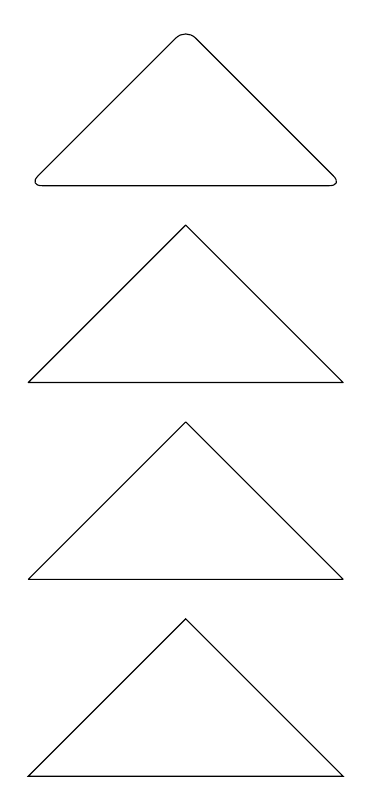
\begin{tikzpicture}
        \draw[line join=mitre] (0,0) -- ++(4,0) -- ++(-2,2) -- cycle; % sharp corner(default)
        \draw[line join=bevel] (0,2.5) -- ++(4,0) -- ++(-2,2) -- cycle;
        \draw[line join=round] (0,5) -- ++(4,0) -- ++(-2,2) -- cycle;
        \draw[rounded corners=5pt] (0,7.5) -- ++(4,0) -- ++(-2,2) -- cycle;
    \end{tikzpicture}

    \newpage

    {\Large Orthogonal Pathways}\\[10pt]
    \begin{tikzpicture}
        \draw (0,0) -| (6,3);
        \draw (8,0) |- (14,3);
    \end{tikzpicture}\\[15pt]

    {\Large Alternate Paths Between Points}\\[10pt]
    % Bending Paths
    % right and left are relative to the straight line path not describing the motion pf the path
    % default curve is symmetric
    \begin{tikzpicture}
        % the size of the curve is define by angle of departure
        % default angle of departure is 30 degree
        \draw (0,0) to[bend left] ++(5,0);
        % 45 degree angle of departure
        \draw (7,0) to[bend right=45] ++(5,0);
    \end{tikzpicture}\\
    % can set In and Out Angles(non-symmetric)
    % 0 degree is point to the right
    \begin{tikzpicture}
        % out to start pt,in to teminal pt
        \draw (0,0) to[out=315,in=135] (5,0);
    \end{tikzpicture}\\[15pt]

    {\Large Transformations}\\[10pt]
    % three transformatin : shift , scale ,rotate
    % can apply t draw,node,circle and several other commands
    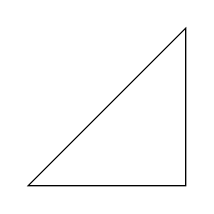
\begin{tikzpicture}
        \draw (0,0)--(2,0)--(2,2)--cycle;
    \end{tikzpicture}
    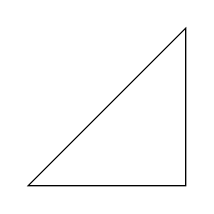
\begin{tikzpicture}
        % shift origin ,not the anchor point of image
        \draw[shift={(2,1)}] (0,0)--(2,0)--(2,2)--cycle;
    \end{tikzpicture}
    \begin{tikzpicture}
        % scale in same ratio,or can use xscale or yscale to scale object separately
        \draw[scale=2] (0,0)--(2,0)--(2,2)--cycle;
    \end{tikzpicture}
    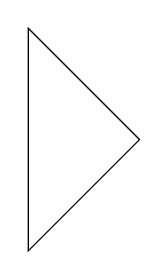
\begin{tikzpicture}
        % rotate about origin not around anchor point,unit degree
        \draw[rotate=45] (0,0)--(2,0)--(2,2)--cycle;
    \end{tikzpicture}

    % the order of transformation is important(non-commutative)
    % tikz execute command from right to left
    % ex : \draw[shift,rotate] = \draw(shift(rotate()))
    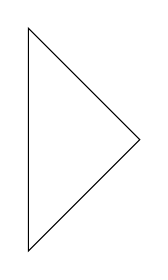
\begin{tikzpicture}
        \draw[shift={(150,0)},rotate=45] (0,0)--(2,0)--(2,2)--cycle;
    \end{tikzpicture}\\
    % its looks same but location are different
    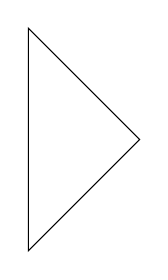
\begin{tikzpicture}
        \draw[rotate=45,shift={(150,0)}] (0,0)--(2,0)--(2,2)--cycle;
    \end{tikzpicture}\\[15pt]

    {\Large Node Border}\\[10pt]
    % if change the node color wiil also change the color of text unless use he \textcolor command inside the node
    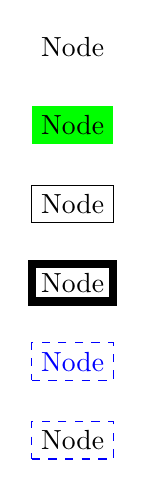
\begin{tikzpicture}
        \draw (0,0) node {Node}
              (0,-1) node[fill=green] {Node}
              (0,-2) node[draw] {Node} % draw option make node border
              (0,-3) node[draw,line width=3pt] {Node}
              (0,-4) node[draw,dashed,blue] {Node}
              (0,-5) node[draw,dashed,blue] {\textcolor{black}{Node}};
    \end{tikzpicture}\\[15pt]

    {\Large Node Placement}\\[10pt]
    % the value 0 corresponds to first coordinate and value 1 corresponds to second coordinate
    % for -- and arc can think as a linear progression
    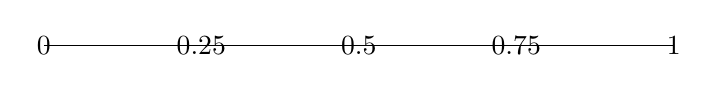
\begin{tikzpicture}
        \draw(0,0)--(8,0)
            node[pos=0]{0}
            node[pos=0.25]{0.25}
            node[pos=0.5]{0.5}
            node[pos=0.75]{0.75}
            node[pos=1]{1};
    \end{tikzpicture}
    \begin{tikzpicture}
        \draw(0,0) arc[radius=4,start angle=180,end angle=0]
            node[pos=0]{0}
            node[pos=0.25]{0.25}
            node[pos=0.5]{0.5}
            node[pos=0.75]{0.75}
            node[pos=1]{1};
    \end{tikzpicture}

    % for orthogonal path the value 0.5 will corresponds to the corner
    % it let the speed along the two paths may not be equal
    \begin{tikzpicture}
        \draw(0,0)-|(8,2)
            node[pos=0]{0}
            node[pos=0.25]{0.25}
            node[pos=0.5]{0.5}
            node[pos=0.75]{0.75}
            node[pos=1]{1};
    \end{tikzpicture}
    % if choose numbers outside of the interval from 0 to 1
    % latex will extrapolate the position based on the path 
    % that dose not work with "to" command
    \begin{tikzpicture}
        \draw(0,0)--(4,0)
            node[pos=-0.5]{-0.5}
            node[pos=0]{0}
            node[pos=0.5]{0.5}
            node[pos=1]{1}
            node[pos=1.5]{1.5};
    \end{tikzpicture}

    \newpage

    % Part3

    % Node is far more flexible objects and we put text,tabular,image,even a tikzpicture ...
    {\Large Math in Nodes}\\[10pt]
    % default is inline mode,can force in display mode but still should present like inline mode
    % because display mode needs to know the width of the page for center the text properly 
    % and default behavior for node is to strech to fit its contents
    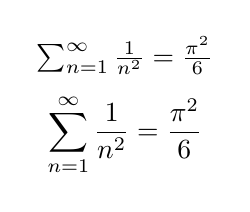
\begin{tikzpicture}
        \draw (0,0) node{
            $\sum_{n=1}^\infty \frac{1}{n^2} = \frac{\pi^2}{6}$
        };
        \draw (0,-1) node{
            $ \displaystyle \sum_{n=1}^\infty \frac{1}{n^2} = \frac{\pi^2}{6}$
        };
    \end{tikzpicture}\\[15pt]

    {\Large Setting the Nodes Text Width}\\[10pt]
    % default is left justified
    % when user define the width ,can use display mode math
    \begin{tikzpicture}
        \draw(0,0) node[text width=6cm]{
            \[\sum_{n=1}^\infty \frac{1}{n^2} = \frac{\pi^2}{6}\]
        };
    \end{tikzpicture}\\[15pt]

    {\Large Drawing a Graph}\\[10pt]
    % prefer using PGF plots because it's more robust approach
    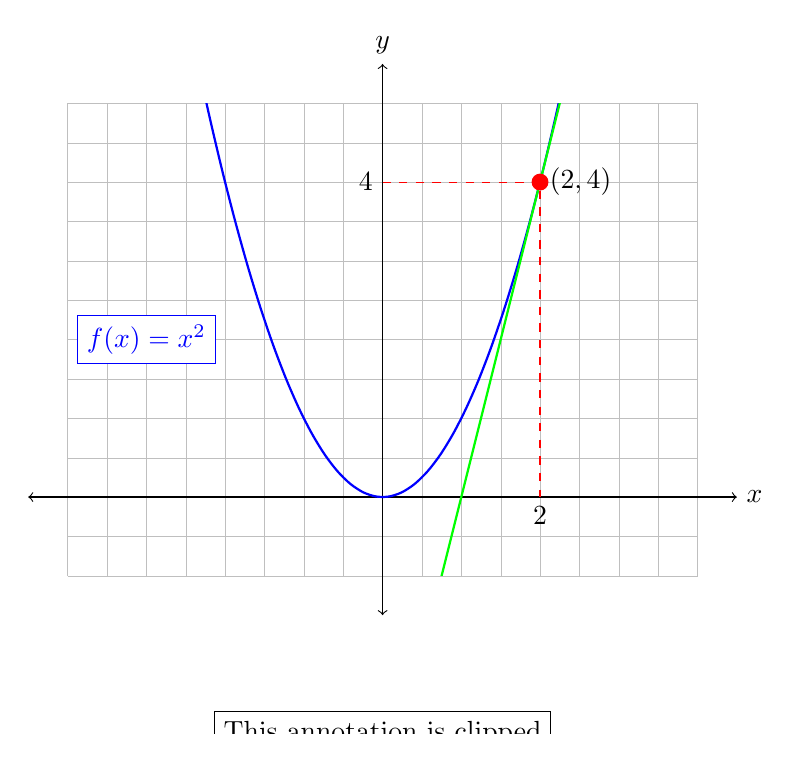
\begin{tikzpicture}
        % display the grid of coordinate
        \draw[ultra thin,lightgray] (-4,-1) grid[step=0.5] (4,5);
        % x-axis
        \draw[<->] (-4.5,0)--(4.5,0) node[right]{$x$};
        % y-axis
        \draw[<->] (0,-1.5)--(0,5.5) node[above]{$y$};

        % to cut the graph that over the grid range
        % the shape can be any closed figure including polygon and circle
        % but we only need to cut the the plot ,use clip will let contents out of range not display
        % we can use scope environment to fix this problem
        % scope environment is drawn on its own and then insert into the larger picture
        % if have complex objects and want to move as a group,
        % we can apply transformations to scope is which handy
        \clip (-4,-3) rectangle(4,5);
        \begin{scope}
            \clip (-4,-1) rectangle(4,5);
            % draw graph
            % should define domain and variable(must need "\" in front of variable)
            % sample : sample point
            % smooth : if smaple is enough ,can make curve sooth
            % plot() : is a function,parametic plot y=f(x) ,coordinate x will be parameter
            \draw[domain=-4:4,variable=\x ,samples=50,smooth,blue,thick] plot( {\x},{(\x)^2} );

            % draw tangent line
            % there is NO way to automatically calculatethe tangent line here
            % so we should calculate the equation by hand
            \draw[domain=-4:4,variable=\x ,samples=50,smooth,green,thick] plot( {\x},{4*\x - 4} );
        \end{scope}
        
        % label the graph
        \draw(-3,2) node[draw,blue,fill=white]{$f(x) = x^2$};

        % mark the point
        \draw[red,fill=red] (2,4) circle[radius=1mm]
                                  node[right,black]{$(2,4)$};

        % draw the dash line to marked point
        \draw[red,dashed](0,4) node[black,left]{4} -|
                         (2,0) node[black,below]{2};
        \draw(0,-3) node[draw]{This annotation is clipped};
    \end{tikzpicture}

    \newpage

    {\Large More Graphs}\\[10pt]
    % functions plot can use : sin(),cos(),tan(),exp(),ln(),abs()
    \begin{tikzpicture}
        \draw[domain=-4:4,variable=\x ,samples=50,smooth,blue,thick]
        %                       deg -> rad 
            plot( {\x},{sin(\x*180/3.14159)} );
    \end{tikzpicture}\\[15pt]

    {\Large For Loops}\\[10pt]
    % the variables can be used both in the coordinate and as text objects
    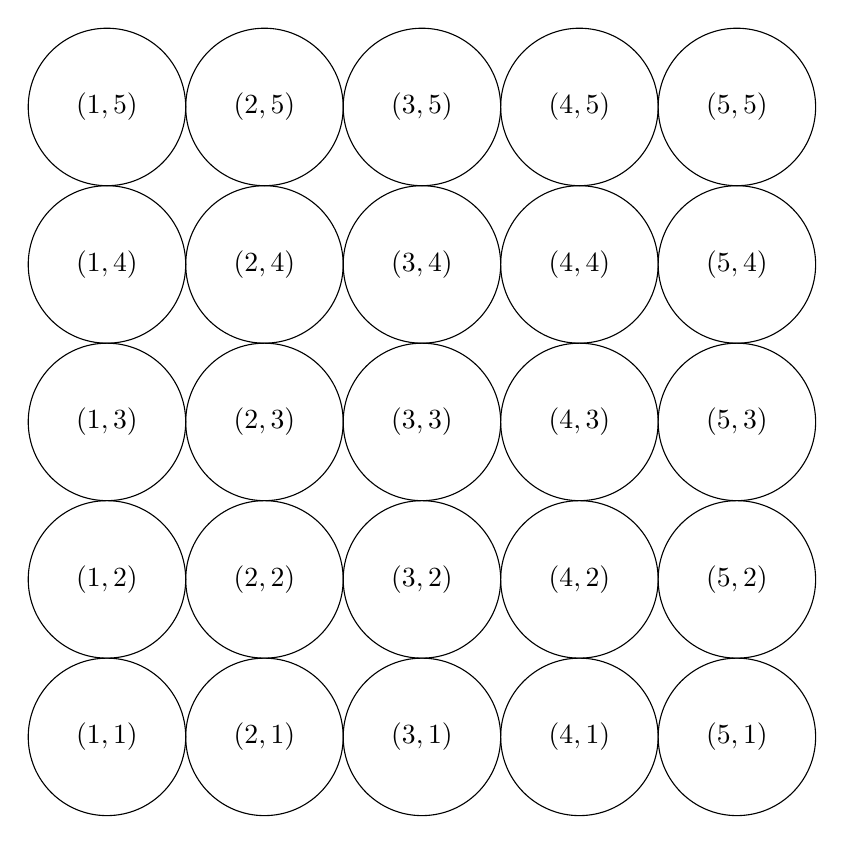
\begin{tikzpicture}
        \foreach \x in {1,2,...,5}{
            \foreach \y in {1,2,...,5}{
                \draw(2*\x,2*\y) circle[radius = 1]
                                 node[anchor=center]{$(\x,\y)$};
            };
        };
    \end{tikzpicture}\\[15pt]

    \newpage

    {\Large Fancy Shading}\\[10pt]
    % tikz is able to color regions using a color gradient instead of a solid color
    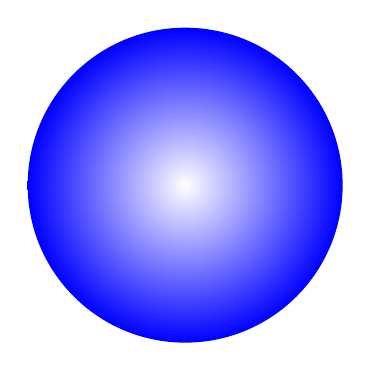
\begin{tikzpicture}
        \shade[shading=radial,inner color=white,outer color=blue] (0,0) circle (2);
    \end{tikzpicture}
    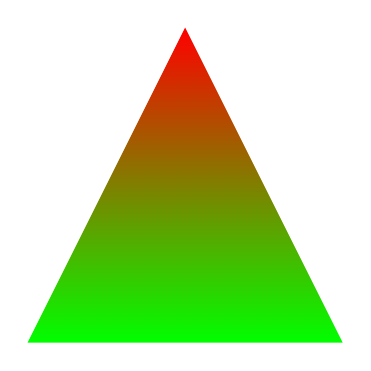
\begin{tikzpicture}
        \shade[top color=red,bottom color=green] (0,0) -- (4,0) -- (2,4)--cycle;
    \end{tikzpicture}\\[15pt]

    {\Large Opacity}\\[10pt]
    % opacity is measure of how well you can see through an image
    % apply on overlaying objects on top of each other without completely hiding everything
    % so much more including 3D coordinate system,fancy node diagrams, mind maps and tree
    % tikz has a method to export diagrams and graphs to geogebra
    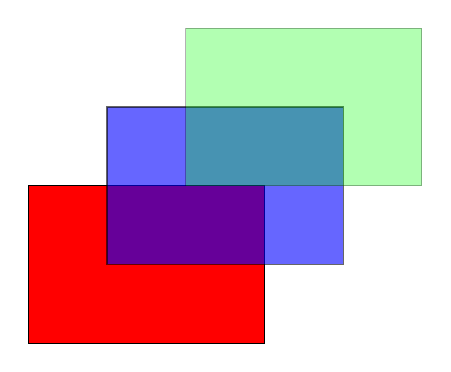
\begin{tikzpicture}
        \draw[fill=red](0,0) rectangle (3,2);
        \draw[fill=blue,opacity=0.6](1,1) rectangle (4,3);
        \draw[fill=green,opacity=0.3](2,2) rectangle (5,4);
    \end{tikzpicture}\\[15pt]
    {\Large Going Further in TikZ}\\[10pt]
    The TikZ manual is very large!\\
    {\LARGE http://www.texample.net/tikz/examples/}
\end{document}